\begin{landscape}
\section{Anhang: Gleichungssysteme und zugehörige Schaltpläne}
\subsection{Würfel}

\subsubsection{Spannung an der Raumdiagonalen}
\begin{align}
\begin{pmatrix}
R_1+R_2+R_3+R_4 &  -R_4  &  0  &  -R_3  &  -R_2  &  0  \\ 
-R_4 & R_4+R_6+R_7+R_{10} & -R_{10} & -R_7 & -R_6 & -R_6 \\ 
 0  & -R_{10} & R_9+R_{10}+R_{11}+R_{12} & -R_{11} & -R_9 & -(R_9+R_{12}) \\ 
-R_3 & -R_7 & -R_11 & R_3+R_7+R_8+R_{11} & 0 & 0 \\ 
-R_2 & -R_6 & -R_9 & 0 & R_2+R_5+R_6+R_9 & R_6+R_9 \\ 
 0  & -R_6 & -(R_9+R_{12}) &  0  & R_6+R_9 & R_6+R_9+R_{12}
\end{pmatrix}
\begin{pmatrix}
I_1\\I_2\\I_3\\I_4\\I_5\\I_{ges}
\end{pmatrix}
=
\begin{pmatrix}
0\\0\\0\\0\\0\\U
\end{pmatrix}
\label{eqn:wuerfel_ganz}
\end{align}
\thispagestyle{empty}
\begin{figure}[htbp!]
\centering
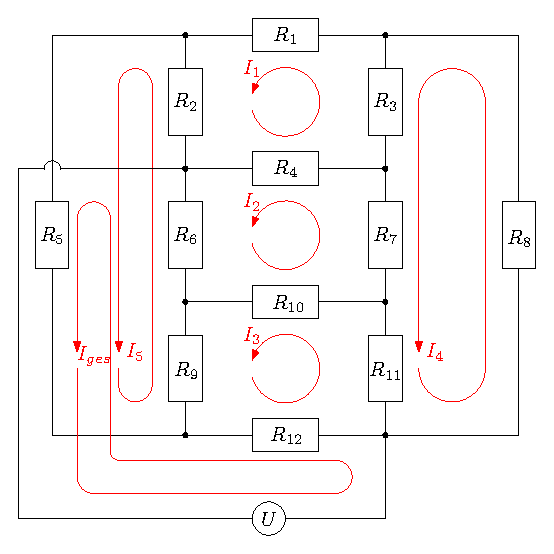
\includegraphics{./figures/wuerfel_schaltplan.eps}
\caption{Schaltplan eines Widerstandswürfels mit angelegter Spannung an einer Raumdiagonalen}
\label{fig:wuerfel_schaltplan}
\end{figure}

\subsubsection{Spannung an der Flächendiagonalen}

\begin{align}
\begin{pmatrix}
R_1+R_2+R_3+R_4 &  -R_4  &  0  &  -R_3  &  -R_2  &  0  \\ 
-R_4 & R_4+R_6+R_7+R_{10} & -R_{10} & -R_7 & -R_6 & -R_6 \\ 
 0  & -R_{10} & R_9+R_{10}+R_{11}+R_{12} & -R_{11} & -R_9 & -R_9 \\ 
-R_3 & -R_7 & -R_11 & R_3+R_7+R_8+R_{11} & 0 & 0 \\ 
-R_2 & -R_6 & -R_9 & 0 & R_2+R_5+R_6+R_9 & R_6+R_9 \\ 
 0  & -R_6 & -R_9 &  0  & R_6+R_9 & R_6+R_9
\end{pmatrix}
\begin{pmatrix}
I_1\\I_2\\I_3\\I_4\\I_5\\I_{ges}
\end{pmatrix}
=
\begin{pmatrix}
0\\0\\0\\0\\0\\U
\end{pmatrix}
\label{eqn:wuerfel_flaeche}
\end{align}
\thispagestyle{empty}

\begin{figure}[htbp!]
\centering
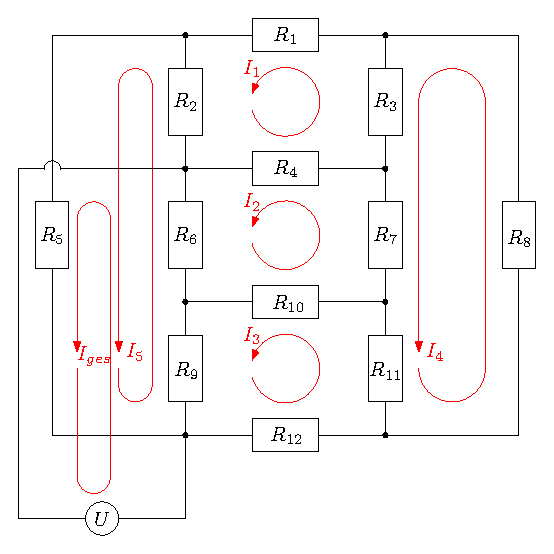
\includegraphics{./figures/wuerfel_schaltplan_flaeche.eps}
\caption{Schaltplan eines Widerstandswürfels mit angelegter Spannung an einer Flächendiagonalen}
\label{fig:wuerfel_schaltplan_flaeche}
\end{figure}

\subsubsection{Spannung an einer Kante}
\begin{align}
\begin{pmatrix}
R_1+R_2+R_3+R_4 &  -R_4  &  0  &  -R_3  &  -R_2  &  0  \\ 
-R_4 & R_4+R_6+R_7+R_{10} & -R_{10} & -R_7 & -R_6 & 0 \\ 
 0  & -R_{10} & R_9+R_{10}+R_{11}+R_{12} & -R_{11} & -R_9 & -R_{12} \\ 
-R_3 & -R_7 & -R_11 & R_3+R_7+R_8+R_{11} & 0 & 0 \\ 
-R_2 & -R_6 & -R_9 & 0 & R_2+R_5+R_6+R_9 & 0 \\ 
 0  & 0 & -R_{12} &  0  & 0 & R_{12}
\end{pmatrix}
\begin{pmatrix}
I_1\\I_2\\I_3\\I_4\\I_5\\I_{ges}
\end{pmatrix}
=
\begin{pmatrix}
0\\0\\0\\0\\0\\U
\end{pmatrix}
\label{eqn:querfel_kante}
\end{align}
\thispagestyle{empty}
\begin{figure}[htbp!]
\centering
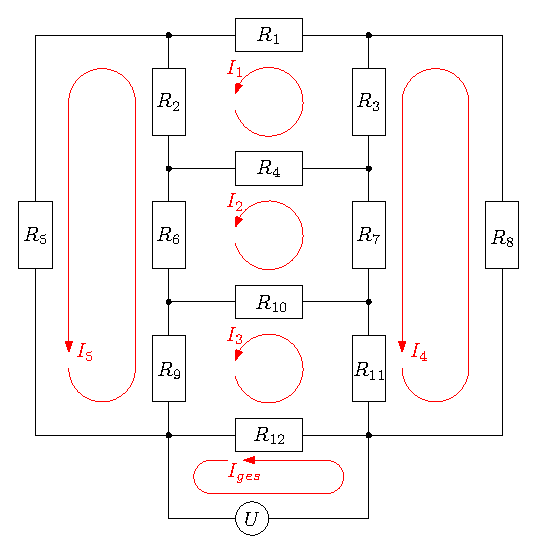
\includegraphics{./figures/wuerfel_schaltplan_kante.eps}
\caption{Schaltplan eines Widerstandswürfels mit angelegter Spannung an einer Kante}
\label{fig:wuerfel_schaltplan_kante}
\end{figure}
\subsection{Oktaeder}

\subsubsection{Spannung an der Raumdiagonalen}
\begin{align}
\begin{pmatrix}
	0 & 0 & -R_4 & 0 & 0 & -R_{12} & 0 & R_4 + R_{12} \\
	R_1 + R_2 + R_5 & -R_2 & 0 & -R_5 & 0 & 0 &-R_5 & 0 \\
	-R_2 & R_2 + R_3 + R_6 & -R_3 & 0 & -R_6 & 0 & -R_6 & 0 \\
	0 & -R_3 & R_3 + R_4 + R_7 & 0 & 0 & -R_7 & -R_7 & -R_4 \\
	-R_5 & 0 & 0 & R_5 + R_9 + R_{10} & -R_{10} & 0 & R_5 & 0 \\
	0 & -R_6 & 0 & -R_{10} & R_6 + R_{10} + R_{11} & -R_{11} & R_6 & 0 \\
	0 & 0 & -R_7 & 0 & -R_{11} & R_7 + R_{11} + R_{12} & R_7 & -R_{12} \\
	-R_5 & -R_6 & -R_7 & R_5 & R_6 & R_7 & R_5 + R_6 + R_7 + R_8 & 0
\end{pmatrix}
\begin{pmatrix}
I_1\\ I_2\\ I_3\\I_4\\I_5\\I_6\\I_7\\I_{ges}
\end{pmatrix}
=
\begin{pmatrix}
U\\0\\0\\0\\0\\0\\0\\0
\end{pmatrix}
\label{eqn:oktaeder_ganz}
\end{align}
\begin{figure}[htbp!]
\centering
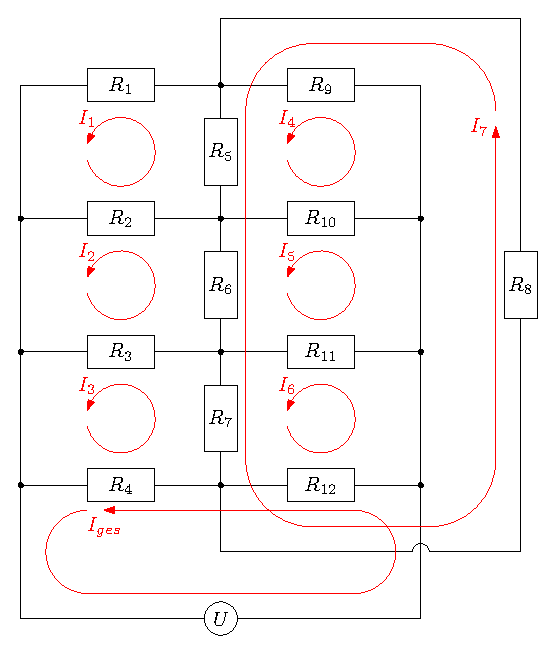
\includegraphics[height=290pt]{./figures/oktaeder_schaltplan.eps}
\caption{Schaltplan eines Oktaeders mit angelegter Spannung an der Raumdiagonalen}
\label{fig:oktaeder_schaltplan}
\end{figure}
\thispagestyle{empty}
\subsubsection{Spannung an einer Kante}

\begin{align}
\begin{pmatrix}
	0 & 0 & -R_4 & 0 & 0 & 0 & 0 & R_4 \\
	R_1 + R_2 + R_5 & -R_2 & 0 & -R_5 & 0 & 0 &-R_5 & 0 \\
	-R_2 & R_2 + R_3 + R_6 & -R_3 & 0 & -R_6 & 0 & -R_6 & 0 \\
	0 & -R_3 & R_3 + R_4 + R_7 & 0 & 0 & -R_7 & -R_7 & -R_4 \\
	-R_5 & 0 & 0 & R_5 + R_9 + R_{10} & -R_{10} & 0 & R_5 & 0 \\
	0 & -R_6 & 0 & -R_{10} & R_6 + R_{10} + R_{11} & -R_{11} & R_6 & 0 \\
	0 & 0 & -R_7 & 0 & -R_{11} & R_7 + R_{11} + R_{12} & R_7 & 0 \\
	-R_5 & -R_6 & -R_7 & R_5 & R_6 & R_7 & R_5 + R_6 + R_7 + R_8 & 0
\end{pmatrix}
\begin{pmatrix}
I_1\\ I_2\\ I_3\\I_4\\I_5\\I_6\\I_7\\I_{ges}
\end{pmatrix}
=
\begin{pmatrix}
U\\0\\0\\0\\0\\0\\0\\0
\end{pmatrix}
\end{align}
\thispagestyle{empty}
\begin{figure}[htbp!]
\centering
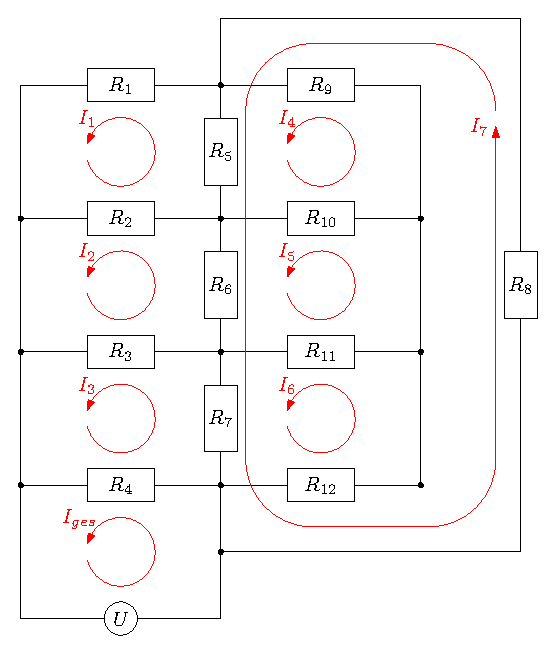
\includegraphics[height=290pt]{./figures/oktaeder_schaltplan_kante.eps}
\caption{Schaltplan eines Oktaeders mit angelegter Spannung an einer Kante}
\label{fig:oktaeder_schaltplan_kante}
\end{figure}
\end{landscape}